\documentclass[11pt,a4paper]{article}

\usepackage{amsmath,amsthm,amsfonts,amssymb}
\usepackage{color, graphicx, pstricks, pifont}
\usepackage{wasysym,marvosym}
\usepackage{fancybox}
\usepackage{epsfig}
\usepackage{booktabs}
\usepackage{rotating}

%\usepackage[table]{xcolor}


\newcommand{\trans}{^{\operatorname{T}}}

\newcommand{\dyeitred}{\textcolor{red}}{}
\newcommand{\dyeitgreen}{\textcolor{green}}{}

\newcommand{\water}{\operatorname{H_2O}}
\newcommand{\elemoxygen}{\operatorname{O}}
\newcommand{\elemhydrogen}{\operatorname{H}}
\newcommand{\hydrogen}{\operatorname{H_2}}
\newcommand{\oxygen}{\operatorname{O_2}}
\newcommand{\hydroxide}{\operatorname{OH}}

\newcommand{\diag}{\operatorname{diag}}



\title{Dimension Reduction of Stiff Systems}
\author{MF}

\begin{document}
\setlength{\parindent}{0pt}

\maketitle

\section{Reduction of source term for isothermal 6-species $\hydrogen$ mechansim -- i.e. 1st approximation}

\textbf{\textsf{Subject: Evaluation of manifold at each function call}}

\bigskip
\textbf{\textsf{General set-up (througout)}} -- reduce 6 species onto 2:  \\
For \texttt{ComputeManifold<double,6,2,true>} take:
\begin{itemize}
  \item rpv index: $0, 4$
  \item order of rpvs: $\hydrogen, \water$
  \item rpv start values: $0.3, 0.6$ 
  \item time horizon: $[t_0,T] = [0.0, 0.2]$
\end{itemize}

\textbf{\textsf{Jochen's tool:}} In \textit{MoRe\_examples/H2C6/SETTING/general\_settings.dat} set:
\begin{itemize}
  \item \texttt{<method> \\ s}
\end{itemize}

\ding{182}\textbf{st Testcase:}\\
\textbf{\textsf{Initial value (IV)}} for solution of ODE (on manifold):\\
 $ u_0(t_0) = [\dyeitred{0.4549999999992859}, 0.7780585738931507, 0.2366143850825262, \\ 0.3628298037265891, \dyeitred{0.1479999999999196}, 0.01594142610843904]\trans$ \\
(The red dyed numbers correspond to starting values of the reduced ODE)\\
\textbf{\textsf{Solution of of full ODE}} (via implicit Euler with stepsize control due to Johnson, Nie, Thom\'ee):\\
$u^*(T) = [0.3786723144539595, 0.04850834768192609, 0.1884211778006195, \\0.01922020051004056, 0.5902095795214345, 0.01372786436728766 ]\trans$\\
%Time: $0.04$ secs.\\
\textbf{\textsf{Solution of reduced ODE}} (via classical adaptive Runge-Kutta-Fehlberg (show this by default)):\\
$u^*(T)_{\mathrm{red}} = [ 0.3623960518126658, 0.6046053938719057 ]\trans$

\begin{center}
  \begin{tabular}{|c|c|c|c|c||c|}
    \hline 
    \textbf{solver} &  \textbf{time [secs]} & \textbf{$\ell_2$-error} & \textbf{slowdown} & \textbf{tol(s)} &\textbf{figure}\\
\hline \hline
implicit Euler & 128.16 & 0.0230448 & 6408 & 1.e-04/1.e-03 &1\\
runge-kutta-fehlberg &3.22 & 0.021729 & 82.25 &  1.e-04 &2 \\
\hline
  \end{tabular}
\end{center}

\begin{figure}
  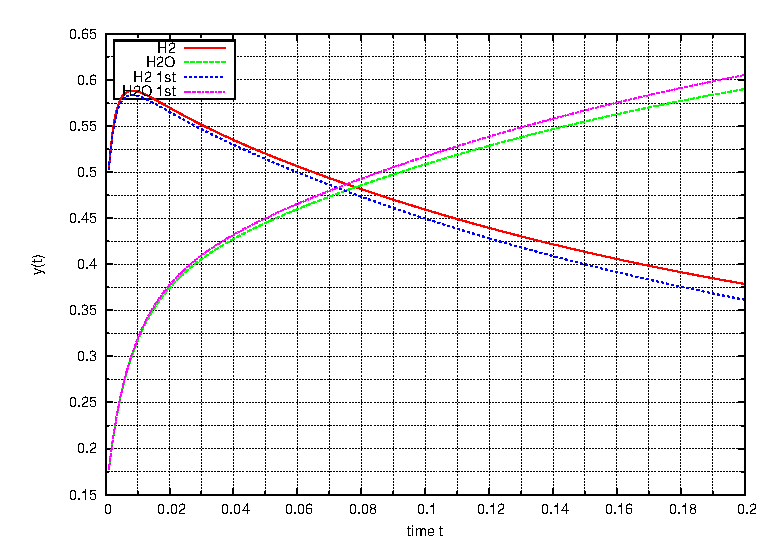
\epsfig{file=implEul1.eps,scale = 1}
  \caption{Reduced vs full temporal evolution -- implicit method}
\end{figure} 

\begin{figure}
  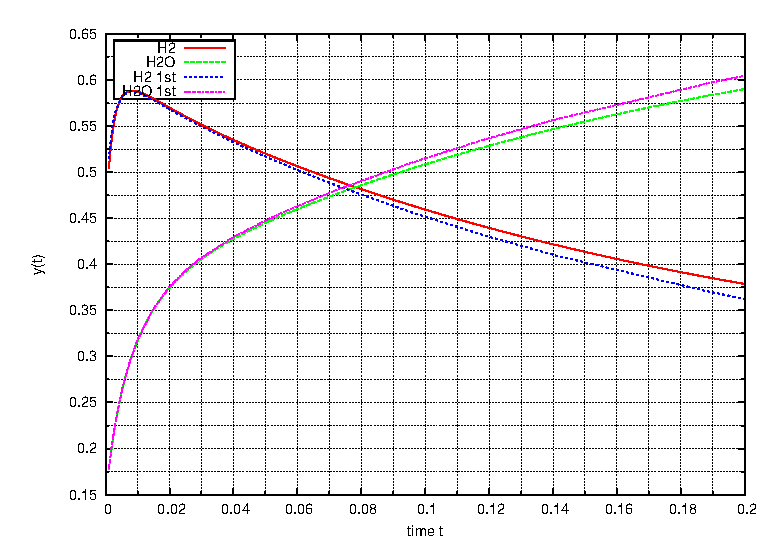
\epsfig{file=rkf1.eps,scale = 1}
  \caption{Reduced vs full temporal evolution -- explicit method}
\end{figure} 


\ding{183}\textbf{nd Testcase:}\\
\textbf{\textsf{Initial value (IV)}} for solution of ODE (on manifold near to equilibrium):\\
 $ u_0(t_0) = [\dyeitred{0.3}, 0.1894550821939027, 0.1437566945658673, \\0.101941693062168, \dyeitred{0.6}, 0.01054491780609743]\trans$\\
(The red dyed numbers correspond to starting values of the reduced ODE)\\
\textbf{\textsf{Solution of of full ODE}} (via implicit Euler with stepsize control due to Johnson, Nie, Thom\'ee): \\
$u^*(T) = [ 0.285310199565836, 0.04976927314406539, 0.1425291708195627, \\0.01987354660256563, 0.6845422159659538, 0.01052589579235477 ]\trans$\\
%Time: $0.01$ secs.\\
\textbf{\textsf{Solution of reduced ODE}} (via classical adaptive Runge-Kutta-Fehlberg (show this by default)):


$u^*(T)_{\mathrm{red}} = [ 0.2553611536492239, 0.7095534070528229 ]\trans$
\begin{center}
  \begin{tabular}{|c|c|c|c|c||c|}
    \hline 
    \textbf{solver} &  \textbf{time [secs]} & \textbf{$\ell_2$-error} & \textbf{slowdown} & \textbf{tol(s)} &\textbf{figure}\\
\hline \hline
implicit Euler & 31.38 & 0.0387793 & 3138 & 1.e-04/1.e-03 &3\\
runge-kutta-fehlberg &1.8 & 0.039019 & 180 &  1.e-04 &4 \\
\hline
  \end{tabular}
\end{center}

\begin{figure}
  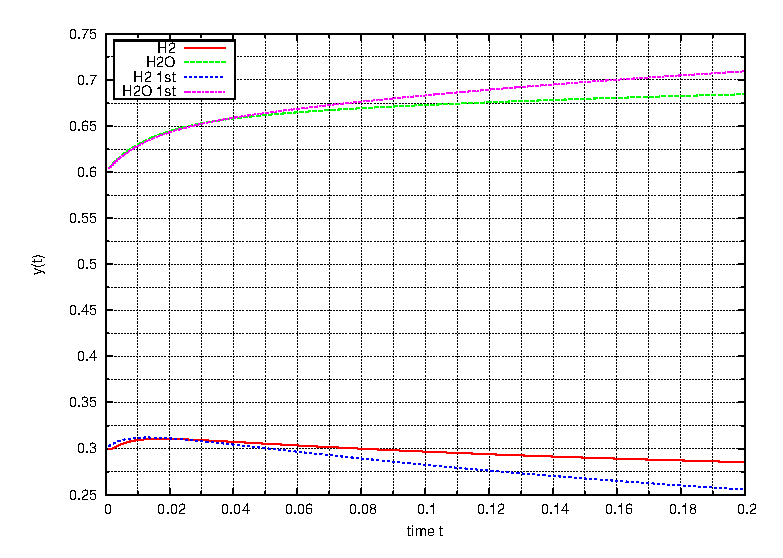
\epsfig{file=implEul2.eps,scale = 1}
  \caption{Reduced vs full temporal evolution -- implicit method}
\end{figure} 

\begin{figure}
  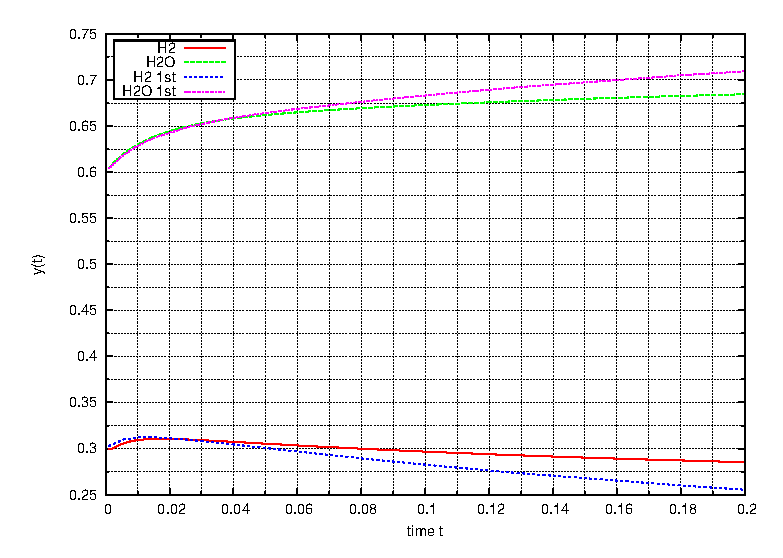
\epsfig{file=rkf2.eps,scale = 1}
  \caption{Reduced vs full temporal evolution -- explicit method}
\end{figure} 

\section{1D Manifold -- Is one species capable of fitting all?}
Finally, it seems that reducing 6 species onto a single one (either $\hydrogen$ or $\water$) doesn't yield good results (see figures beneath). This may result from the fact that one species (or in particular one of the aforementioned) are not capable of simulating the complete system within reasonable accuracy.

 \begin{figure}
  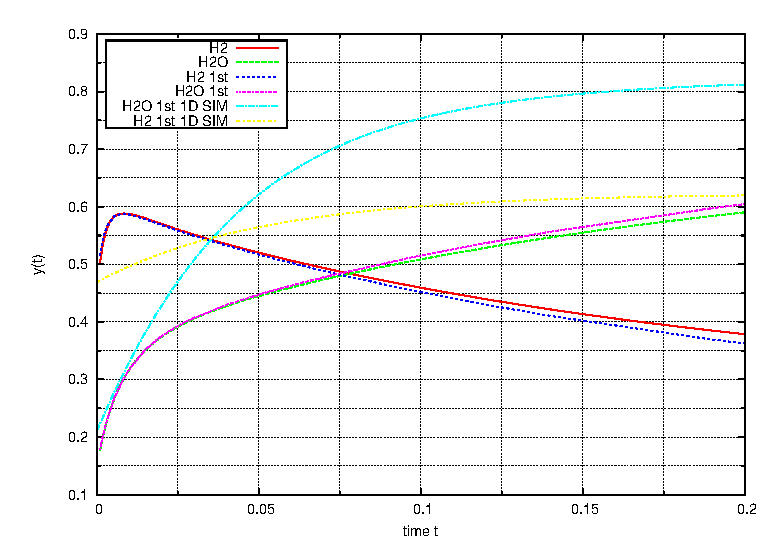
\epsfig{file=simulationwith1dSIM_awayfromequi.eps,scale = 1}
  \caption{The above figure, completed by simulating only one species ($\hydrogen$ and $\water$, respectively)}
\end{figure} 

\begin{figure}
  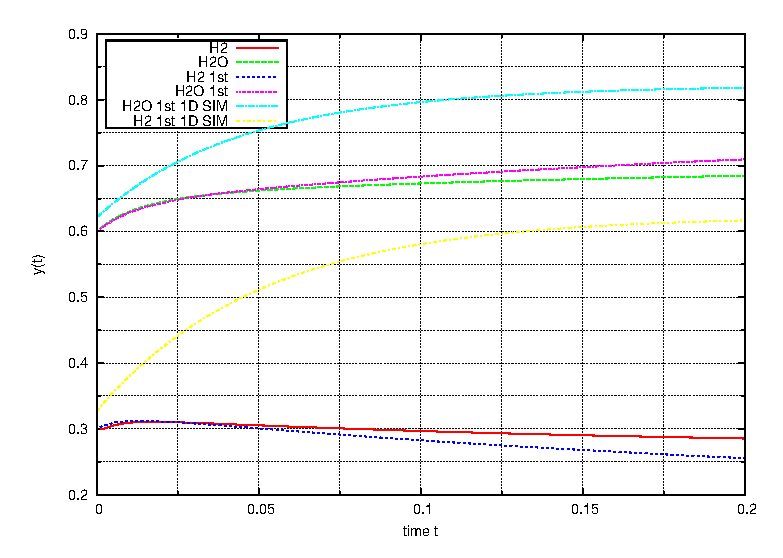
\epsfig{file=simulationwith1dSIM_nearequi.eps,scale = 1}
  \caption{The above figure, completed by simulating only one species ($\hydrogen$ and $\water$, respectively) -- this time with starting values near the equilibrium.}
\end{figure} 

\section{Solution over long time interval}
In order to verify that the solution doesn't depart further, once the time horizion gets larger, we simulated the temporal evolution once again with the same settings as before, except that we changed the time horizon into $[0.0, 23.66].$\\
Compared to the solution of the full system\\ $U^*(T=23.66) = 0.269998, 0.0499998, 0.134999, \\ 0.0199999, 0.700002, 0.00999992 ]\trans$, the solution of the rteduction is \\ $u^*(T=23.66)_{\mathrm{red}} = [0.205539, 0.756834]\trans $ with $\ell_2 = 0.0859348.$

\begin{figure}
  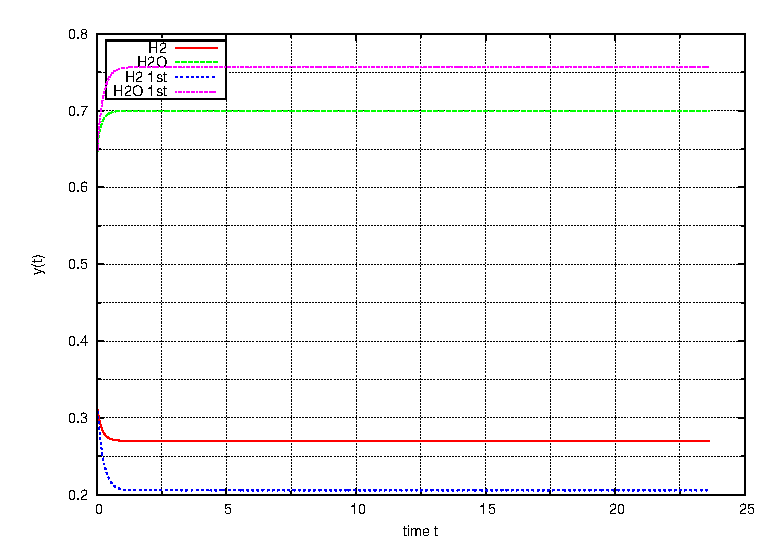
\epsfig{file=longtimeinterval_long.eps,scale = 1}
  \caption{Integration over time horizion $[0.0, 23.66]$ shows that the reduction remains bounded (initial condition was taken to lie further away from equilibrium and similar results are obtained from other ics).}
\end{figure}

Similar results where obtained for even longer time horizons (here $[0., 60]$):\\
$u^*(T=60.) = [ 0.205506, 0.75679 ]$ with $\ell_2 = 0.0859303.$
\begin{figure}
  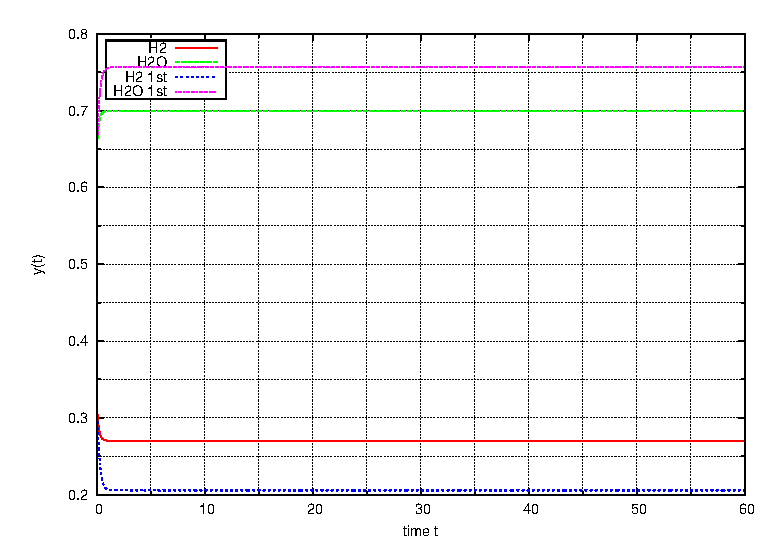
\epsfig{file=longtimeinterval_evenlonger.eps,scale = 1}
  \caption{Integration over time horizion $[0.0, 60.]$.}
\end{figure}


\section{1D Spatio-temporal evolution}

\begin{figure}
  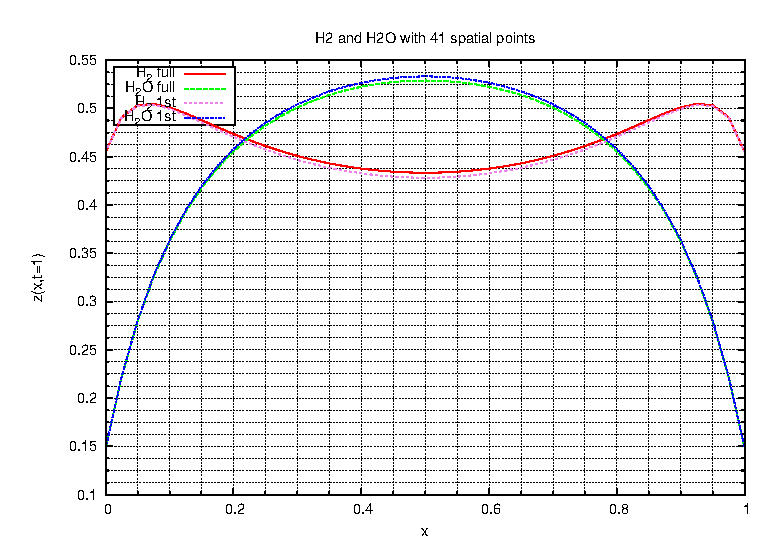
\epsfig{file=Diffusionconst_fullvs1st_tols_1e-03_1e-02_hstep_0.0025.eps ,scale = 1}
  \caption{Original system vs. 1st approximation. Integration has been performed over time horizion $[0.0, 0.2.]$ and with 41 spatial points.}
  \label{fig:diff1d}
\end{figure}

The entries of the inital value vector \\$u(t=0) = [0.4549999999992859, 0.7780585738931507, 0.2366143850825262, \\0.3628298037265891, 0.1479999999999196, 0.01594142610843904]\trans $ have been taken to be \textit{constant} for each spatial grid point.\\Furthermore we assume (somewhat very academic) constant and equal diffusion, i.e. $\mathcal{D} = \diag\{1\}_{i=1,\ldots,6}$. \\
The domain has been choosen to be $\Omega = ]0,1[.$ At $x = 0$ and $x = 1,$ Dirichlet bdy conditions have been assumed, i.e. $U(0,t) = U(1,t) = 0 \forall t \leq 0.$ \\
Invocation of the modelreduction algorithm has been started at \textit{every} function evaluation. The function is just the discretization of the reduced source function via the method of lines.\\
Aside from the fact that the result looks pretty nice, cf. fig. \ref{fig:diff1d}, the running time for the (1st) reduction is rather frightening\ldots

\begin{center}
\begin{tabular}{|c|c|c|c|c|c|c|}
  \hline
 \textbf{system} & \textbf{solver} & \textbf{tol(s)} & \textbf{spatial points} & \textbf{homotopy} &  \textbf{AD} & \textbf{time}  \\
\hline \hline
full & impl. Euler & 1.e-03/1.e-02 & 41 & yes & no& 3.67 secs \\
red. (1st) & impl. Euler& 1.e-03/1.e-02 & 41 & yes & no& 17.40 h\\

\hline
\end{tabular}
\end{center}
\end{document}
